% LM122A Pablo Rodrigo Sanches
\documentclass[12pt,a4paper]{article}
\usepackage[utf8]{inputenc}
\usepackage[onehalfspacing]{setspace}
\usepackage[lmargin=3cm,tmargin=3cm,rmargin=2cm,bmargin=2cm]{geometry}
\usepackage[brazil]{babel}
\usepackage[T1]{fontenc}
\usepackage{fancyhdr}
\usepackage{graphicx}
\usepackage{indentfirst}
\usepackage{comment}
\usepackage{enumerate}
\usepackage{listingsutf8}
\usepackage{xcolor}
\usepackage{pgffor}
\usepackage{hyperref}
\usepackage{tabularx}
\usepackage{subfig}

\definecolor{dkgreen}{rgb}{0,0.6,0}
\definecolor{gray}{rgb}{0.5,0.5,0.5}
\definecolor{mauve}{rgb}{0.58,0,0.82}

\usepackage{hyperref}
\hypersetup{
    colorlinks=true,
    linkcolor=blue,
    filecolor=magenta,
    urlcolor=cyan,
}

\lstset{frame=tb,
  language=C++,
  aboveskip=3mm,
  belowskip=3mm,
  showstringspaces=false,
  columns=flexible,
  basicstyle={\small\ttfamily},
  numbers=none,
  numberstyle=\tiny\color{gray},
  keywordstyle=\color{blue},
  commentstyle=\color{dkgreen},
  stringstyle=\color{mauve},
  breaklines=true,
  breakatwhitespace=true,
  tabsize=8,
  extendedchars=true,
  inputencoding=utf8,
  texcl=true,
}

\lstset{literate=%
{í}{{\'i}}1
{ó}{{\'o}}1
{ú}{{\'u}}1
{é}{{\'e}}1
{ê}{{\^e}}1
{á}{{\'a}}1
{ã}{{\~a}}1
{â}{{\^a}}1
{õ}{{\~o}}1
{ô}{{\^o}}1
{ç}{{\c c}}1
}

% numeracao header
\pagestyle{headings}

% quebra de pagina por secao
\let\oldsection\section
\renewcommand\section{\clearpage\oldsection}

\begin{document}

\begin{titlepage}
	\begin{center}
		\textbf{UNIVERSIDADE DE RIBEIRÃO PRETO} \\
			CIÊNCIAS EXATAS \\
			Lógica e Criatividade

			\vspace{1.5cm}

			\textbf{Prof. Pablo Rodrigo Sanches}
			\vspace{0.5cm}

			\textbf{Murilo da Silva Ijanc'} \\
			RA: 834125

			\vspace{6.5cm}

			\textbf{ATIVIDADE PARCIAL}

			\vfill

			\vspace{0.8cm}

			
\includegraphics[width=0.2\textwidth]{unaerp}

			\textbf{RIBEIRÃO PRETO} \\
			\textbf{2020}
	\end{center}
\end{titlepage}


\thispagestyle{empty}

\tableofcontents

\newpage

%\thispagestyle{empty}
%\listoftables
\thispagestyle{empty}
\listoffigures
\thispagestyle{empty}
%\printglossary[type=main,style=long,nonumberlist]

\pagenumbering{arabic}

% secao 1
\section{Decoberta}

\subsection{Sonhos}
\begin{itemize}
	\item Um alarme quando o pet realizassse necessidade;
	\item Um limpador automático quando o pet fizesse suas necessidades;
	\item Recebesse uma mensagem no celular quando meu pet fizessse suas
		necessidades;
\end{itemize}

\subsection{Pesadelos}
\begin{itemize}
	\item A higiene do pet poderia ser mais rápida
		automaticamente;
	\item Meu pet poderia fazer suas necessidades sempre no mesmo lugar;
	\item Meu apartamento poderia ter um cheiro mais agradável;
\end{itemize}

\subsection{Persona A}

\begin{minipage}{0.3\textwidth}
	
\includegraphics[width=5cm]{universitaria}
\end{minipage}%
\hfill%
\begin{minipage}{0.6\textwidth}\raggedleft
	Ana Luísa \\
	27 Anos \\
	Estudante \\
	Mora em um apartamento com seus pets \\
	Tempo limitado entre os estudos
\end{minipage}

\subsection{Persona B}

\begin{minipage}{0.3\textwidth}
	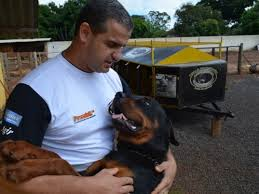
\includegraphics[width=5cm]{canil}
\end{minipage}%
\hfill%
\begin{minipage}{0.6\textwidth}\raggedleft
	Lucas Silva \\
	38 Anos \\
	Adestrador \\
	Mora no mesmo local que possui o canil com a sua família \\
	Passa o dia treinando e realizando propaganda do seu canil
\end{minipage}


\subsection{Persona C}

\begin{minipage}{0.3\textwidth}
	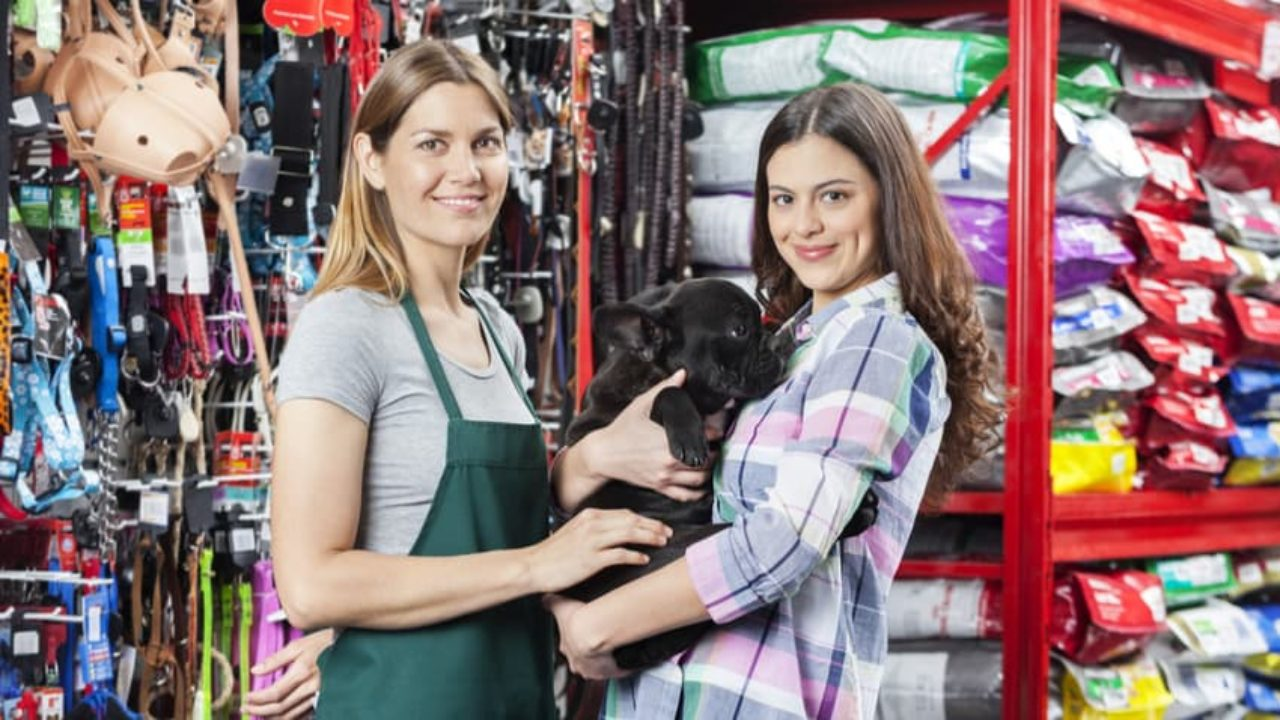
\includegraphics[width=4cm]{dono_petshop}
\end{minipage}
\hfill
\begin{minipage}{0.6\textwidth}\raggedleft
	Mônica Almeida\\
	41 Anos \\
	Donta Petshop\\
	Ligada a tecnologia mônica sempre buscas \\
	novas tendências como diferencial para o seu petshop.
\end{minipage}

\section{Interpretação}
Em ambientes pequenos como apartamentos os pets realizam suas necessidades
diárias próximo aos seus donos, exigindo uma maior atenção para manter o
ambiente higienizado e com cheio agradável. Qualquer demora na higienização
pode acarretar problemas irreversíveis para o ambiente, bem como para o pet
e seus donos.

\begin{figure}[htb!]
	\centering
	\subfloat[Foto Higienização 1]{{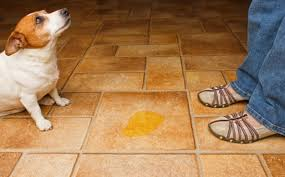
\includegraphics[width=5cm]{pipi_imgs/higienizacao1}}}
	\qquad
	\subfloat[Foto Higienização 2]{{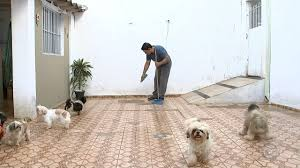
\includegraphics[width=5cm]{pipi_imgs/higienizacao3}}}
	\qquad
	\subfloat[Foto Higienização 3]{{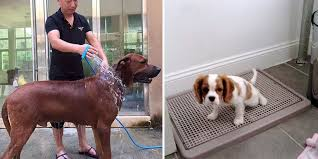
\includegraphics[width=5cm]{pipi_imgs/higienizacao2}}}
	\caption{Foto Higienização}
	\label{fig:higienizacao}
\end{figure}

\begin{figure}[htb!]
	\centering
	\subfloat[Foto fralda 1]{{
\includegraphics[width=5cm]{pipi_imgs/frauda1}}}
	\qquad
	\subfloat[Foto tapete 1]{{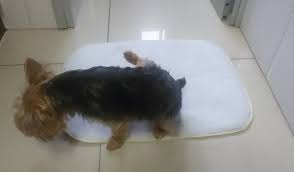
\includegraphics[width=5cm]{pipi_imgs/tapete1}}}
	\qquad
	\subfloat[Foto tapete 2]{{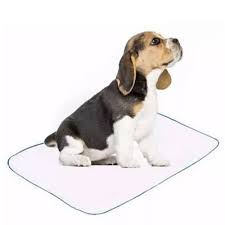
\includegraphics[width=5cm]{pipi_imgs/tapete2}}}
	\caption{Foto Tapete higiênico}
	\label{fig:tapete2}
\end{figure}

\section{Ideação}

\subsection{Rascunho visual}

\begin{figure}[htb!]
	\centering
	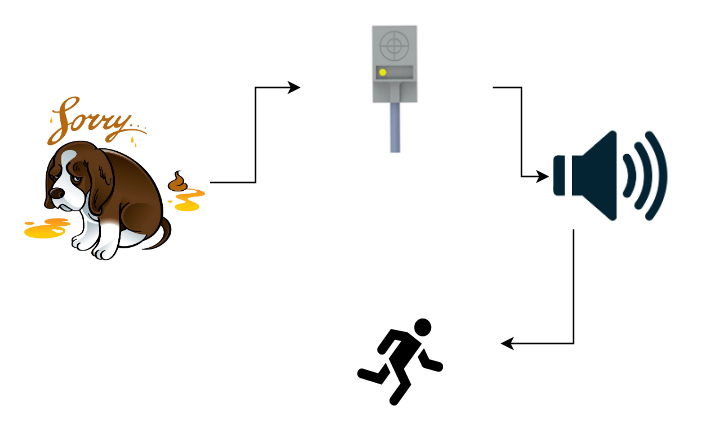
\includegraphics[width=13cm]{fluxograma}
	\caption{PipiPet Fluxograma}
	\label{fig:fluxograma}
\end{figure}

\begin{figure}[htb!]
	\centering
	\subfloat[Tela Boas vindas]{{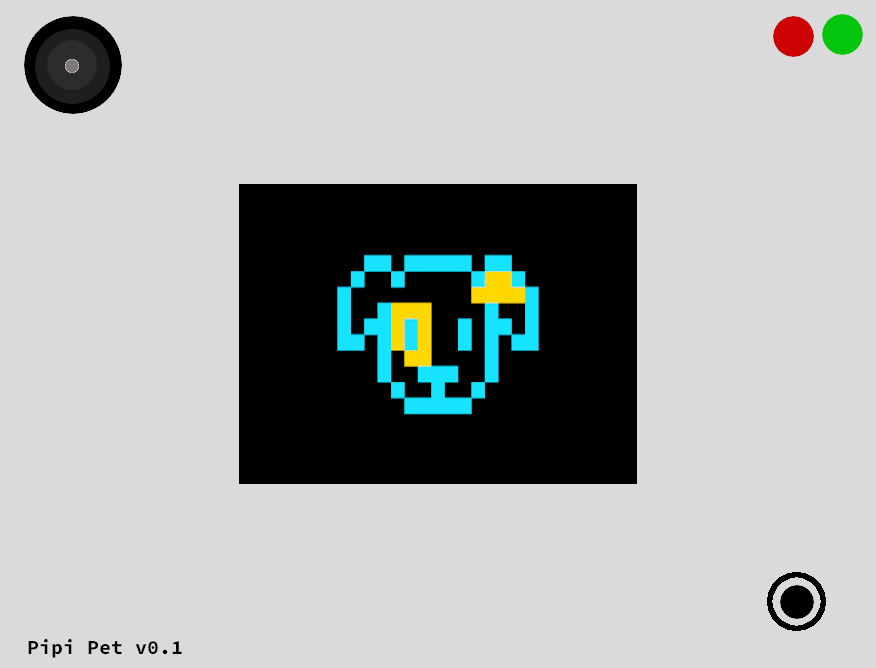
\includegraphics[width=6cm]{interface_1} }}
	\qquad
	\subfloat[Tela Contagem de necessidades]
		{{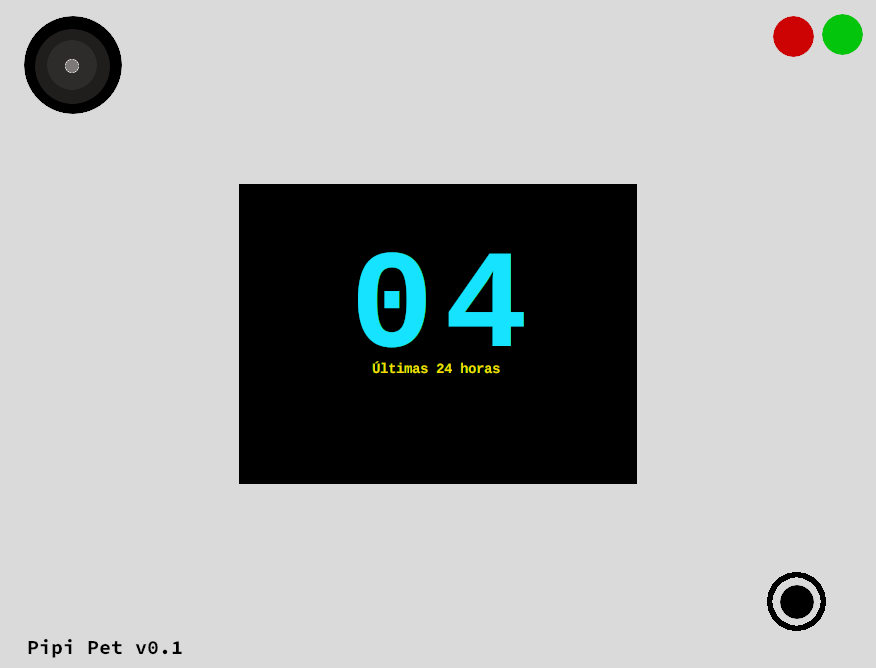
\includegraphics[width=6cm]{interface_2} }}
	\caption{Inteface Pipi Pet}
	\label{fig:interface}
\end{figure}

\subsection{Nome da proposta}
Pipi Pet

\subsection{Como funciona}
Sensor colocado próximo onde o pet realiza as suas necessidades, pode ser
fixado na parede ou na gaiola não mais do que 30cm do pet. Após ligado o
o sensor acende um led verde apontando que o sensor está ligado e operando. O
sensor ultraŝonico fica obtendo a cada 100ms a distância de algum objeto
(\textbf{pet}) uma vez que esse objeto fica a uma distância menor ou igual
20cm o alarme emite um som durante todo o período que o pet realiza suas 
necessidades; um led vermelho também é acesso isso para acesso a pessoas
que tem problemas auditivos quando o pet finalizar o led vermelho é desligado e 
o alarme da busina também.

Observações:
\begin{itemize}
	\item Após as três tentativas sonoras o alarme desliga mas o led vermelho 
		continua aceso;
	\item Através de um botão a pessoa pode desativar o alarme durante o toque do
		mesmo e também apagar a luz, mas as necessidades continuam sendo exibidas
		das últimas 24 horas \textbf{Para o código que possui oled};
	\item A cada 24 horas é resetado o número de necessidades;
\end{itemize}

\subsection{Oportunidades}
\begin{itemize}
	\item Melhora higienização de apartamentos de pequeno a médio porte;
	\item Melhora Higienização gaiolas dos petshops;
	\item Melhora Higienização de canis;
	\item Dificulta a dispersão de odores nos ambientes acima;
\end{itemize}

\subsection{Descrição}
Pipi Pet higienização ao seu controle.

%
% Fotos do tinkcad, prototipagem e link para vídeo
%
\section{Experimentação e evolução}
\subsection{Fotos}
\begin{figure}[htb!]
	\centering
	\includegraphics[width=10cm]{shot2}
	\caption{Sistema Desligado}
	\label{fig:desligado}
\end{figure}

\begin{figure}[htb!]
	\centering
	\includegraphics[width=10cm]{shot3}
	\caption{Sistema Ligado}
	\label{fig:ligado}
\end{figure}

\begin{figure}[htb!]
	\centering
	\includegraphics[width=10cm]{shot5}
	\caption{Sistema Ativado quando há necessidades do pet}
	\label{fig:necessidades}
\end{figure}

\newpage

\subsection{Algoritmo}
O código pode ser visto abaixo ou pelo link \href{
	https://www.tinkercad.com/things/9dnCu8UsG4O}{protótipo pipipet v0.0.1}
\lstinputlisting{main.cpp}

\subsection{Testes}

Abaixo uma lista de itêms que serão relevantes para o sucesso do produto:

\begin{itemize}
	\item Enviar uma mensagem de texto para o celular para atingir longas
		distâncias;
	\item Uso de uma fonte externa em quedas de energia;
	\item Permitir o usuário customizar a distância do sensor ultrasônico;
	\item Ativar automaticamente uma fonte externa de fluxo de água como uma
		torneira, bomba para jogar agua no ambiente logo após o pet realizar a
		necessidade;
\end{itemize}

\end{document}
